\section{商品评论标签爬取}

首先对苏宁网站上的商品网页进行分析,苏宁的域名组织较有规律,这也是我们选它作为目标网站的原因之一。对于商品详情页,其组织形式是“https://product.suning.com/\{\}/\{\}.html.format(shop, sku)”,其中shop是10位的一串商铺代号,如苏宁自营是“0000000000”。后面的sku是11位的商品代号,如Apple Watch是“11357287387”。

整体来说,实现苏宁商品评价的思路和京东的类似,主要差别就在于上面的参数由京东的一个商品productID变为了苏宁的商铺ID和商品ID。那么将爬虫的处理商品评价的函数改为双参数即可。
\begin{python}
def crawl_sn_cmt_tag(sku, shop):# change for url
\end{python}

然而还有一个不同是,苏宁的评价内容,标签,以及统计信息放在三个不一样的url。我们通过上面京东部分介绍过的寻找请求url的方法可以分别找到对应的目标url。

通过采取上一节中寻找京东商品评价标签类似的方法,我们找到了苏宁商品评价标签的位置,如图\ref{img:yhb111}所示。

\begin{figure}[htbp]
\centering
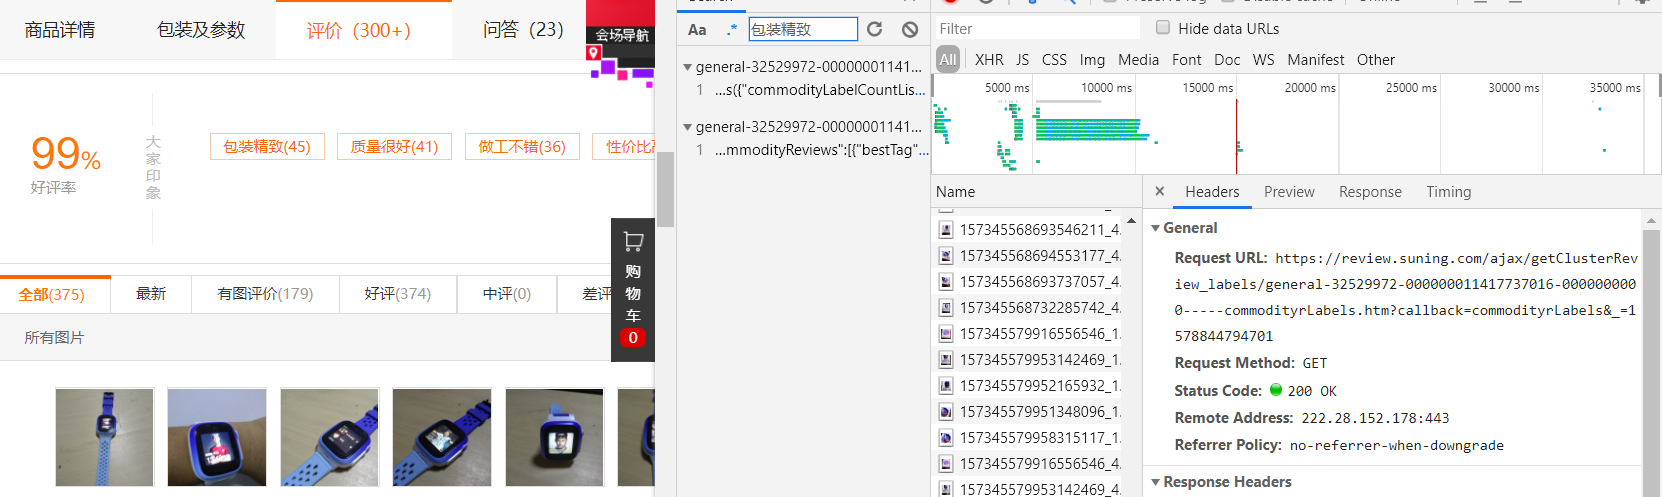
\includegraphics[width=13.5cm]{img/yhb/sn_eg2.png}
\caption{获取苏宁评价标签的请求地址}
\label{img:yhb111}   % 引用标记,用于文章中引用
\end{figure}

抽取商铺和商品ID得到:
\begin{python}
url=r"https://review.suning.com/ajax/" \
        r"getClusterReview_labels/cluster-33667504-0000000" \
        r"{}-{}" \
        r"-----commodityrLabels.htm?".format(sku,shop)
\end{python}


经过试验,我们发现cluster之后的一串数字在请求地址中扮演类似时间戳的作用,对爬取内容不产生影响,因此我们在这里直接忽略对该串数字的考虑即可。在调用json库转换对象之后,面临的问题就和之前在京东解决过的一模一样了。对京东标签的代码稍加修改即可。这里需要注意的是,有些商品ID不足11位,需要进行补足:
\begin{python}
while (len(sku) < 11):
                sku = "0" + sku
\end{python}


爬取结果示例如图\ref{img:yhb100}所示。

\begin{figure}[htbp]
\centering
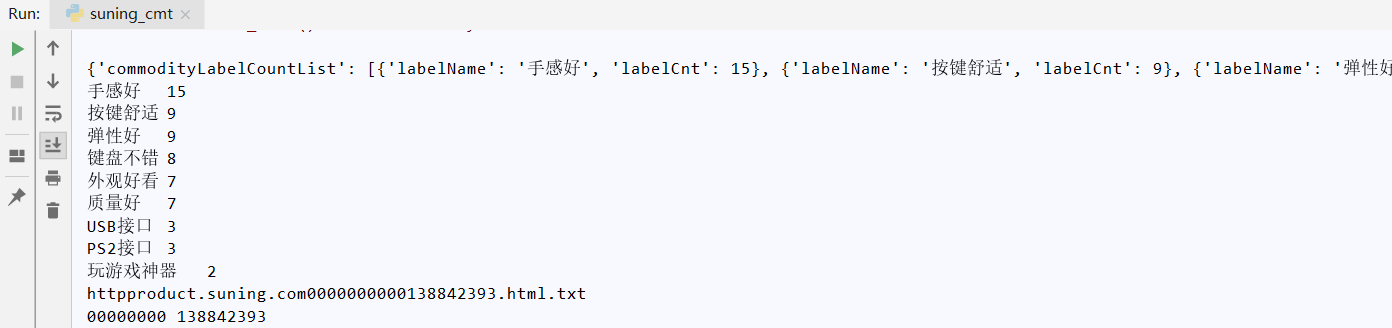
\includegraphics[width=13.5cm]{img/yhb/sn_res1.png}
\caption{爬取苏宁商品评论标签的结果}
\label{img:yhb100}   % 引用标记,用于文章中引用
\end{figure}

\section{商品评分计算}

采用上一节中所述类似的方法,我们定位了苏宁评论区上方统计信息的请求地址,如图\ref{img:yhb121}所示。

\begin{figure}[htbp]
\centering
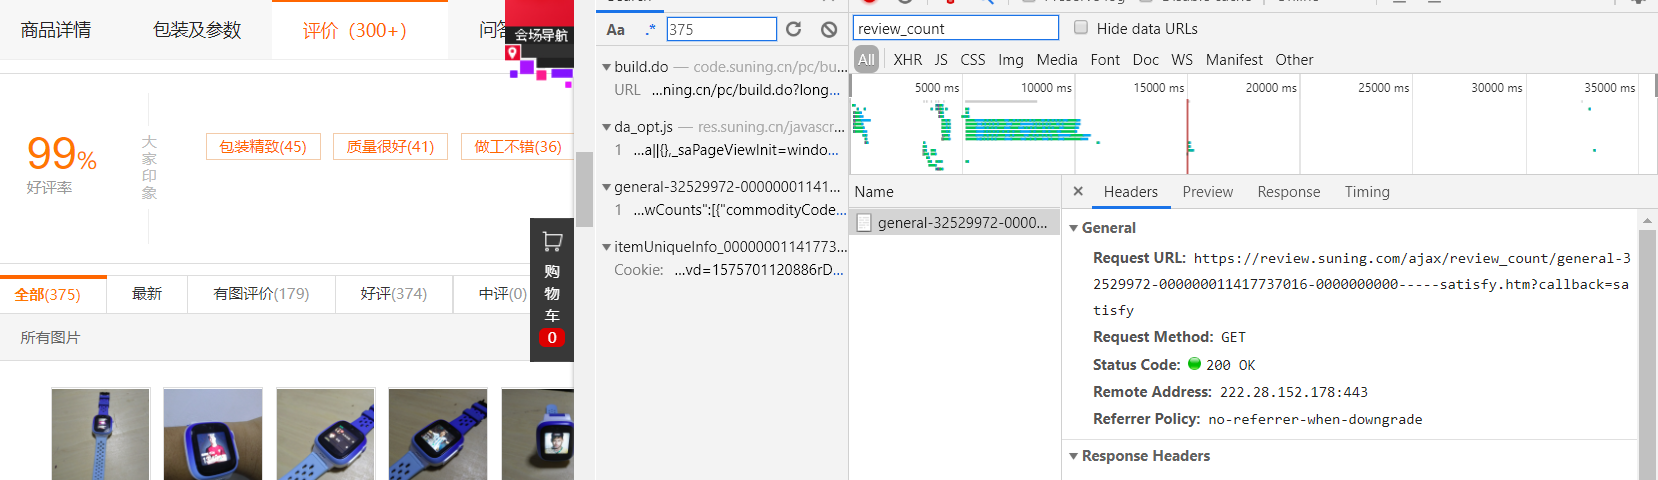
\includegraphics[width=13.5cm]{img/yhb/sn_eg.png}
\caption{评论统计信息的请求地址}
\label{img:yhb121}   % 引用标记,用于文章中引用
\end{figure}

抽取商铺和商品ID得到:
\begin{python}
url=r"https://review.suning.com/ajax/" \
        r"review_count/cluster-32762695-0000000" \
        r"{}-{}" \
        r"-----satisfy.htm?".format(sku,shop)
\end{python}

采用上文同样的方法,我们可以给出商品的评分。评分结果示例如图\ref{img:yhb101}所示。

\begin{figure}[htbp]
\centering
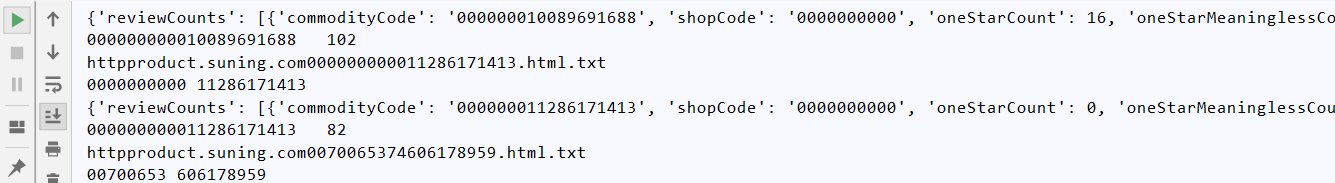
\includegraphics[width=13.5cm]{img/yhb/sn_res2.png}
\caption{商品评分结果示例}
\label{img:yhb101}   % 引用标记,用于文章中引用
\end{figure}

以上就是京东和苏宁爬虫的全部内容了,到这里我们已经完成了所有信息的准备和预处理的工作。




